\chapter{A3}

{\LARGE 'Determine the 50 most popular IP addresses external to the domain by number of bytes.'}

\section{Explicação do código desenvolvido}

Se compararmos com os outros códigos, a computação deste talvez seja considerada a mais simples. Isto não pela sua complexidade por si só, mas pela semelhança com o código em A2. No fundo, a única entre os dois devesse só a onde, nos ficheiros csv, ir buscar o resultado. Observe-se no código abaixo, que os \textit{bytes} são conseguidos na coluna 10 do ficheiro.

\begin{figure}[h!]
    \label{high}
    \centering
    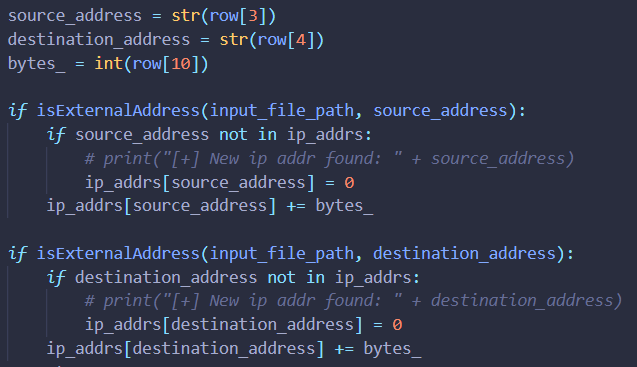
\includegraphics[width=0.9\textwidth]{Images/a3/a3.png}
    \caption{\textit{Código do tópico a3}}
\end{figure}

%----------------------------------------------------------------------------
%----------------------------------------------------------------------------

\newpage

\section{Resultados obtidos pelo ficheiro www.fct.unl.pt.csv}

Como  se  pode  ver  na  figura  4.3,  foram  processadas  as  linhas do ficheiro www.fct.unl.pt.csv, tendo ordenado, por número de bytes, os endereços IP.

\begin{figure}[h]
    \label{high}
    \centering
    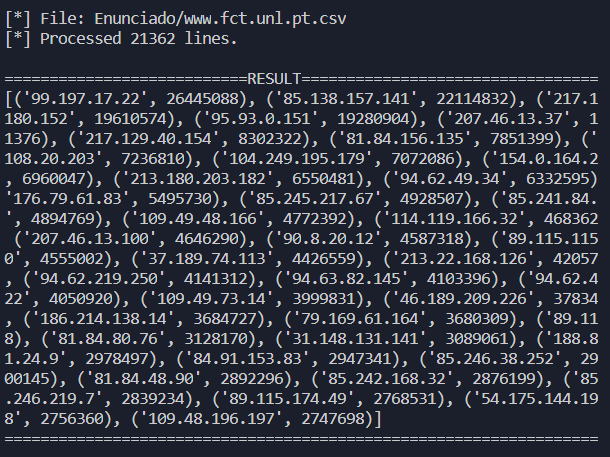
\includegraphics[width=1\textwidth]{Images/a3/a3_a.png}
    \caption{\textit{Output do script a3.py}}
\end{figure}

%----------------------------------------------------------------------------

\section{Resultados obtidos pelo ficheiro bigFlows.csv}

Como  se  pode  ver  na  figura  4.4,  foram  processadas  as  linhas do ficheiro bigFlows.csv, tendo ordenado, por número de bytes, os endereços IP.

\begin{figure}[h]
    \label{high}
    \centering
    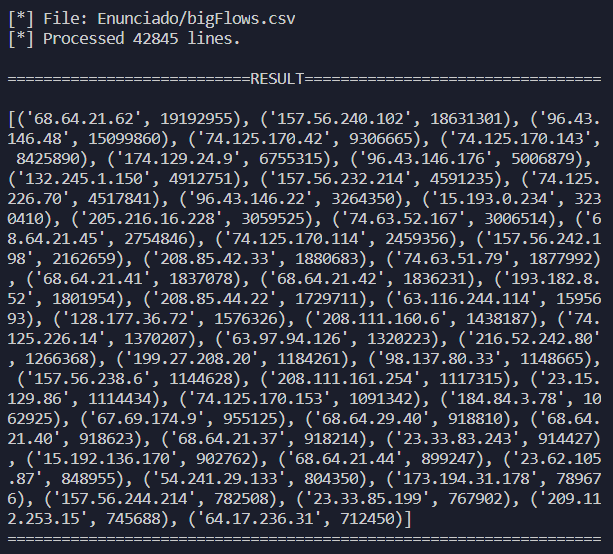
\includegraphics[width=1\textwidth]{Images/a3/a3_b.png}
    \caption{\textit{Output do script a3.py}}
\end{figure}
\par
Este exercício foi realizado de forma quase igual ao anterior, sendo a única diferença que em vez de nos vermos o flow, vimos o número de bytes como foi pedido.